%%%%%%%%%%%%%%%%%%%%%%%%%%%%%%%%%%%%%%%%%%%%%%%%%%%%%%%%%%%%%%%%%%%%%%%%%%%%%%%
\documentclass[english,a4paper,11pt]{ieee}
\usepackage{times}
\usepackage[T1]{fontenc}
\usepackage{babel}
\usepackage{url}
\usepackage{graphicx}
\usepackage[latin1]{inputenc}

\title{MPEG hardware decoder implementation: is domain decomposition the best approach?}

\author{Ronaldo H�semann, Ad�o de Souza Junior\\
        UNIVATES University Center, Lajeado, RS, Brazil\\
        Valter Roesler\\
        Federal University of Rio Grande do Sul\\
        {rhusemann, adao, valter.roesler}@gmail.com\\
        Danillo Moura Santos, Ant�nio Augusto Fr�hlich\\
        Federal University of Santa Catarina\\
        Laboratory for Software and Hardware Integration\\
        {danillo, guto}@lisha.ufsc.br\\
}

\begin{document}

\maketitle
\thispagestyle{empty}

%-------------------------------------------------------------------------------
\begin{abstract}

Usual domain engeneering and decomposition identifies components that will compose a system. These components are identifyed based on previous domain knowledge. Most system design methodologies like AOSD (Application-Oriented System Design) assumes that these components (implemented in software or hardware) are the best way to design complex applications. This paper presents a fast hardware implementation of the computational part of a MPEG decoder algorithm with HDTV 1080i processing capabilities, that couldn't be obtained following domain decomposition process. This implementation is compared to an implementation obtained using domain engineering to decompose the system in already known components in terms of area cost and performance, exposing its cost-benefit relationship. We discuss why AOSD methodology have not helped the designer in perceiving  parallel hardware characteristics separated in two or more components.

\paragraph{Keywords:} embedded systems, MPEG-2 decoder, methodology

\end{abstract}

%-------------------------------------------------------------------------------
\section{Introduction}

The development of complex embedded systems is feasible due to the low cost provided by the technology advance. This complexity is also present in the design process. The Computer-Aided Design~(CAD) tools evolution has aided this process. Embedded systems design methodologies is a hot research topic nowadays, the establishment of a good methodology would reduce the development time of new systems and make easier the reuse of components developed in different designs.

Hardware/Software Co-design methodologies, such as IP-Based Design~(IBD)~\cite{Gajski:1999} and Platforma-Based Design~(PBD)~\cite{Vincentelli:2001}, despite the name, barely solve software design issues comparably to modern software engineering methodologies. The main focus of current co-design methodologies seems to be on the design of a hardware platform for a given application domain, on top of which some software will be running. The software itself, is mostly regarded as application programmer's duties. Furthermore, the guidelines to decompose an application domain in IPs that will eventually build up a platform are mostly empirical.

The \emph{Application-Oriented System Design}~(AOSD) methodology~\cite{Frohlich:2001} was developed to build component-based run-time support systems that can be tailored according to the requirements of particular applications. This methodology guides the developer, from design to implementation, to produce an application-oriented system. 
By this, we mean that this system will match exactly the requirements of a specific application. This methodology uses good software engineering techniques, such as Domain Analysis and Decomposition, Family Based Design~(FBD)~\cite{Parnas:1976} and Aspect Oriented Programming~(AOP)~\cite{Kiczales:1997} to separate abstractions from scenario dependent aspects (hardware and environment dependencies). Abstractions are free to reuse and extend, and are independent from a scenario execution.

While trying to combine Application-Oriented System Design with Platform-Based
Design~(PBD) to produce a comprehensive embedded systems design methodology, we concluded that the main concepts behind PBD, i.e. an \emph{application programming interface} and an \emph{architecture}, were already promptly addressed by AOSD. Therefore, we assumed that AOSD is indeed able to guide the complete development of embedded systems~\cite{Polpeta:2005}. In 2004, the PDSCE project was setup to investigate exactly that\footnote[1]{The Project PDSCE -- Embedded Systems Development Environment is funded by FINEP under grant no. 01.04.0903.00}. Supporting tools were extended to cover hardware component demands, the concept of "Hardware Mediator" evolved into a powerful software/hardware interface mechanism, and several embedded systems were developed. 

In this paper, we discuss one case study, a MPEG-2 High Definition~(HD) decoder developed in the scope of the Brazilian Digital Television Project~(SBTVD). During this system development, we realized that the ordinary domain decomposition techniques have failed in identifying parallel hardware characteristics, wich were implicit in different hardware components. Therefore, we propose a new approach for a fast hardware implementation that performs the computational part of MPEG decoder algorithm, which includes Huffmann entropy decoding, inverse scan, inverse quantization and IDCT, with HDTV 1080i processing capabilities.

This paper is organized as follows: Section~\ref{aosd_overview} shows the AOSD methodology, used in the decoder design, Section~\ref{case_study} presents the MPEG-2 decoder algorithm and the proposed implementation, Section~\ref{results} compares the proposed approach to the traditional decoder algorithm, and finally, in the conclusion we discuss why the best solution was not identified during AOSD domain decomposition.

%-------------------------------------------------------------------------------
\section{AOSD Overview}
\label{aosd_overview}

Application-Oriented System Design~(AOSD) is a domain engineering methodology that
elaborates on the well-known domain decomposition strategies behind Family-Based
Design~(FBD) and Object-Orientation~(OO), i.e. \emph{commonality} and
\emph{variability} analysis, to add the concept of \emph{aspect} identification and
separation yet at the early stages of design~\cite{Frohlich:2001}. In this way, AOSD
guides a domain engineering towards families of components, of which execution
scenario dependencies are factored out as "aspects" and external relationships are
captured in a component framework. This domain engineering strategy consistently
addresses some of the most relevant issues in component-based software development:
\begin{itemize}

\item Reusability: components tend to be highly reusable, for they are modeled as
abstractions of real elements of a given domain and not as parts of a target system.
Moreover, by factoring out execution scenario dependencies as aspects, components
can be reused unmodified in a variety of scenarios simply by defining new aspect
programs.

\item Complexity management: the identification and separation of execution scenario
dependencies implicitly reduces the number of components in each family, since those
components that would have been modeled to express a variation in the domain that
originates from a scenario dependency are suppressed whenever the dependency can be
modelled as an aspect. Simply stated, a set of 100 components could be modeled as a
set of 10 or more components plus a set of aspects and a mechanism to apply aspects to
components. The overall complexity (and functionality) in the new set of 100
generated components is the same, but it is now confined in fewer constructs. These
directly improves on maintainability.

\item Composability: by capturing component relationships in a component framework,
AOSD enables components to be more easily combined while generating a system
instance. It also put some limits to the misbehaviors that can arise from applying
aspect programs to pre-validated components. \emph{Feature-based models} are of great value at this point to capture configuration knowledge and thus make system generation a more predictable procedure.

\end{itemize}

Hardware mediators were initially created to facilitate the portability of applications and run-time support systems developed following AOSD methodology through different hardware platforms (microcontrollers or personal computers).

The main idea of this portability artifact is to keep an \emph{interface contract} between the operating system and the hardware. Each hardware component is accessed through its own mediator, thus granting the portability of abstractions that use it without creating unnecessary dependencies.

Software components can be implemented in hardware if its interface is kept. The mediator, in this case, invokes the hardware respective to the routine early implemented in software. This allows the developer to choose wich implementation to use according to the application requirements, in the case of processing hungry applications, as the MPEG decoder, a hardware implementation can be done without much effort.

%-------------------------------------------------------------------------------
\section{Case Study: MPEG-2 Decoder}
\label{case_study}

Most of the current digital multimedia devices use MPEG video compression to code and decode video information. MPEG algorithms aim at reducing the amount of data by exploiting the video spatial and temporal redundancy. Images where only the spatial redundancy is subject to reduction are compressed as intra frame (i-frames). Such frames are by their turn used as references to predicted or bidirectional frames (p or b-frames) where both spatial and temporal redundancies are targeted. 

To cope with frame rates of up to 19Mbps, MPEG High-Definition decoders (1920x1080 pixels) may demand a full hardware implementation. In fact, even using a hardware approach to perform real time decoding of high definition videos, design optimization is imperative to achieve a fast and reliable solution at feasible cost.

The next sections shows the computational part of MPEG decoder algorithm developed according to AOSD domain decomposition, which resulted in a component-based system. This system is composed by Huffmann entropy decoding, inverse scan, inverse quantization and IDCT, with HDTV 1080i processing capabilities. The first implementation was a complete software solution, then some software components were implemented in hardware using VHDL~(Very High Speed Integrated Circuit Hardware Description Language) to satisfy application performance demand as shows the section~\ref{traditional_approach}.

A novel optimized architecture to the implementation of the computational modules of MPEG decoder is presented in section~\ref{proposed_approach}. The increase in the processing speed of the computational module have a direct impact in the overall performance of the decoder. A comparison between the implementations can be seen at section~\ref{results}.

%-------------------------------------------------------------------------------
\subsection{Traditional approach}
\label{traditional_approach}

Figure \ref{fig:mpeg_straightforward_apprach} presents a simplified structure of a generic MPEG decoder (including MPEG-2 and MPEG-4 standards), identifying its main internal modules. The input module is responsible by receiving data from communication channel, generating a video Elementary Stream (ES) in a bit oriented format. ESD (Elementary Stream Decoder) analyses the received ES in order to separate parameter information from compressed video data. There are two kinds of data: video data, which is routed to the computational module to be directly decompressed, and motion vectors, which are passed to motion compensation module to recover video frames using temporal information.

\begin{figure*}[!hbt]
\begin{center}
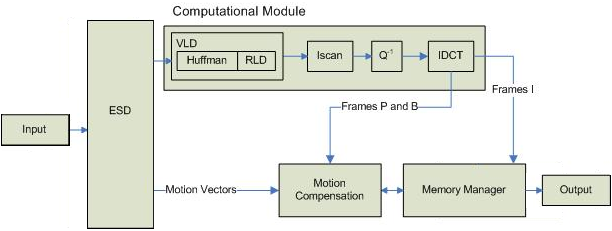
\includegraphics[height=6.11cm,width=16.19cm]{figuras/ieee_decoder.png}
\caption{Basic structure of a MPEG decoder \label{fig:mpeg_straightforward_apprach}}
\end{center}
\end{figure*}

Four blocks with different tasks compose the computational module of the MPEG decoder:

\begin{itemize}

\item Huffman/RLD (Run Length Decoder): receives a variable length Huffman compressed bitstream coded in run/level format and expand it in regular 4x4 or 8x8 pixels matrices (MPEG blocks); 

\item IScan (Inverse Scan): rearranges decompressed data placing the obtained coefficients (levels) in their correct matrix positions; 

\item Iquant (Inverse Quantization) or Q-1: multiplies the  matrix coefficients with predefined factors to recover the approximated original values;

\item IDCT (Inverse Discrete Cosine Transform): uses the generated matrix to recover the luminance and chrominance data.

\end{itemize}

The motion compensation module recovers the original frames using temporal prediction information to operate on the reference images. MPEG supports two kinds of temporal prediction: backward prediction (using previous frames) and forward prediction (using future frames). The block must use the motion vectors information that comes in the bit-stream to perform the macroblock (set of 16x16 pixels) placements that are required in order to obtain the original video frames.

As video processing is a data intensive activity, memory access is performed by a dedicated memory manager, which provides shared accesses for different modules, avoiding memory conflicts and deadlocks. Figure \ref{fig:mpeg_straightforward_apprach} shows this module next to the output block.

The output module collects video information from the decoded frames memory and sends it synchronized with audio information to a TV or monitor. It also converts data to a standard video output format. Some examples of possible output formats are YPbPr (composite video), SDI (Serial Digital Interface), DVI (Digital Video Interface) and HDMI (High-Definition Multimedia Interface).

A traditional approach to the design of MPEG decoders in hardware follows the overall dataflow presented in Figure \ref{fig:mpeg_straightforward_apprach}. In the following sections, a traditional solution for each of the computational modules is presented.

%-------------------------------------------------------------------------------
\subsubsection{VLD (Huffman/ RLD)}

Huffman codes for MPEG video employs a fixed set of  variable length codes to compress the most common run/level tuples. A traditional design uses a finite state machine (Moore FSM) to decode Huffmann codes serially, bit-by-bit as they are arriving in the bit-stream. However, that is an expensive solution, since it consumes many logic cells. Thus hardware implementations normally define an input stage of serial to parallel conversion. Since Huffman codes have variable length, a rather large input register is required to align the code. Once the codes are aligned, decoding is a matter of applying a fixed length table (Aspar, 2000) (see Figure \label{fig:huffman_decoder_structure}).
ls figu 
\begin{figure}[!hbt]
\begin{center}
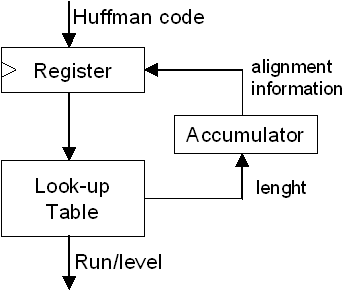
\includegraphics[width=8.1cm]{figuras/huffman_structure.png}
\caption{Huffman decoder structure \label{fig:huffman_decoder_structure}}
\end{center}
\end{figure}

In each run/level tuple, level represents normalized coefficient data, while the run information indicates a sequence of zero values that precedes it. The resulting data is arranged in 4x4 or 8x8 coefficient matrices.

%-------------------------------------------------------------------------------
\subsubsection{Inverse Scan (Q-1)}

During compression process, data in the coefficient matrix is reordered to maximize the length of zero runs in the algorithm. While decoding one must place each coefficient data in its original array position. MPEG defines different scan sequences that one must take into account, for MPEG-2 they are two: zigzag and alternative scan. Traditional approaches implements inverse scan by performing successive read and write operation. In order to reduce processing time, some implementations use distinct data memories in a pipeline arrange (REFER�NCIA).

%-------------------------------------------------------------------------------
\subsubsection{Inverse Quantization}

DCT coefficients must pass for a scaling stage called Iquant before entering the IDCT block. This is required due to quantization in the MPEG compression. In fact, since the encoder implements a lossy compression process, the decoder video will also present a higher amount of error. 

Quantization in MPEG standards uses at least two fixed tables, for intra and non-intra coefficients, but also support custom tables inserted in the stream by the encoder. That characteristic increases the area of any inverse quantizer because demands support for configurable tables. In addition, MPEG standard describes the parameter \emph{Qscale}, which implements an additional control over compression decompression data, like a secondary value of quantization (equation \ref{eq:quantization}).

\begin{equation}
Coef(i,j)=\frac{16 . data( i, j)}{ Qtable( i, j) . Qscale}\label{eq:quantization}
\end{equation}

Any complete MPEG inverse quantizer implementation must consider all these demands. A generic solution must include at least three internal quantization tables, each one with 64 values (two with fixed and one with variable values). From equation \ref{eq:quantization} it is possible to see the need of two stages multipliers in the block (REFER�NCIA).

%-------------------------------------------------------------------------------
\subsubsection{Inverse Discrete Cosine Transform}

MPEG uses Discrete Cosine Transform (DCT) to identify spatial redundancy, grouping low frequencies in the matrix left upper corner and thus allowing compression of intra frames. Its inverse method, IDCT (Inverse Discrete Cosine Transform) is implemented in MPEG decoders to reverse the operation. Both transforms are important performance bottlenecks in the overall compression process. For instance, in a typical MPEG decode process, IDCT generally represents 25\% of total operations (REFER�NCIA).

The Discrete Cosine Transform and its inverse algorithm were introduced by Ahmed \cite{AHMED:1974}. The implementation of an IDCT for a one-dimensional vector is given by equation \ref{eq:idct_one_dimensional}, and, for a two-dimensional matrix, in equation \ref{eq:idct_two_dimensional}.

\begin{equation}
x_i=\frac{2}{N}\sum_{a=0}^{N-1} K_a X_a \cos(\frac{(2_i + 1)u\pi}{2N})
\label{eq:idct_one_dimensional}
\end{equation}

\begin{eqnarray}
x_i,_j & = & \frac{1}{4} \sum_{a=0}^7\sum_{v=0}^7 K_u K_v X_a,_v \cos(\frac{(2_i + 1)u\pi}{16}) \nonumber\\ & & x \cos(\frac{(2_i + 1)u\pi}{16})
\label{eq:idct_two_dimensional}
\end{eqnarray}

Since this transform is widely used on image processing, filtering and compression, many algorithms have been proposed in order to minimize its computational cost. A rather common approach is to try decreasing the number of multiplications and stages, presenting solutions for one-dimensional transforms. In MPEG, however, an intra-frame data block is composed by matrices of 4x4 or 8x8 pixels, then, the most common method is to apply an one-dimensional IDCT over the original input matrix, transpose this data results and apply another one-dimensional IDCT. The final data is obtained transposing results of the second 1D-IDCT.

In a paper in 1989, Loeffler \cite{LOEFFLER:1989} introduced a new practical fast method. In his approach, for an 8-point 1D-IDCT, only 11 multiplications and 29 additions are required, and if more precision is necessary, a modification is proposed just adding one multiplication. It increases the number of multipliers, but results in an algorithm with no multiplications in sequence. It also represents a good solution for fixed point architectures.  For such advantages this method was selected for the implementation of the IDCT block. In the proposed approach part of its functionality is divided with a pre-processing block (see section \ref{proposed_approach}).

%-------------------------------------------------------------------------------
\subsection{Proposed approach}
\label{proposed_approach}

In this approach, a single block called decompression module was developed including operations that were usually distributed in more than one block. Figure \ref{fig:mpeg_proposed_approach} depicts the changes made. This allows one to concentrate singular properties of the above algorithms in one optimized module, reducing circuit size and total execution time. Decompression module includes the following functions:

\begin{itemize}

\item VLD: Decoding run/level values in data coefficients;

\item ISCAN: Re-ordering of coefficients to adjust correct positions;

\item IQUANT: Inverse quantization of coefficients matrices,  normalizing its values;

\item Pre-calculation of IDCT: implementation of the first stage of  IDCT calculation. 

\end{itemize}

\begin{figure}[!hbt]
\begin{center}
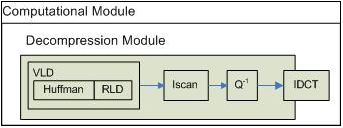
\includegraphics[width=8.1cm]{figuras/ieee_proposed_decoder.png}
\caption{Proposed computational module \label{fig:mpeg_proposed_approach}}
\end{center}
\end{figure}

The following subsections will explore in deeper details the novelties presented in the method.

%-------------------------------------------------------------------------------
\subsubsection{Decompression Module}
\label{decompression_module}

The Decompression module merges multiplication and data positioning operations, as illustrated in Figure \ref{fig:decompressing_module}. Two 8x8 matrices are used to store and process data. While one is being read, the other could be written, allowing continuous operation. These matrices can be adjusted to process 4x4 data as well, for use when the encoder chose this block size.

\begin{figure*}[!hbt]
\begin{center}
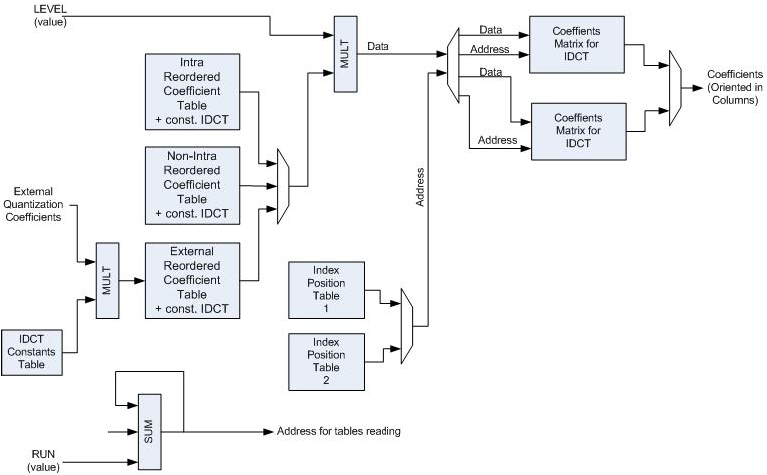
\includegraphics[width=17.2cm]{figuras/proposed_decompressing_module.png}
\caption{Structure of decompressing module \label{fig:decompressing_module}}
\end{center}
\end{figure*}

The first step performed by the decompressing module is to clear (set to zero) all output data coefficients. Therefore each coefficient matrix is formed by an array of registers, cleared in one clock cycle. This approach simplifies the number of operations and allows the reduction of time spent waiting coefficients with value zero during run/level decoding.  

Each block uses current run values to calculate the pointer to an index table, which dictates how many array positions from the current one must be skipped before one writes the next coefficient. This pointer is used to access a specific index position table to calculate the real position in coefficient matrix where the level data will be written. This used strategy implements inverse scan process in parallel with inverse quantization, optimizing the system.

The value to be written in the matrix represents the value in the tupple corresponding to the ``level'' multiplied by a scale factor. Inverse quantization supplies this factor, which is the product of the value assigned by the quantization matrix by the value of qscale. Quantization tables addressed by the same index are used on the input data. There are different possible quantization tables, depending on the corresponding block type. Since the index array already takes scanning into account, data is placed indirectly in the final position to be processed by the IDCT. Besides that, data is arranged already pre-transposed, simplifying the IDCT operation.

%-------------------------------------------------------------------------------
\subsubsection{IDCT Module}
\label{idct_proposed}

The top-level IDCT module, called 2D-IDCT is subdivided in three parts, as shown in Figure \label{fig:idct_module}. In data path, the first module performs a Loeffler 1D-IDCT. The input data is directly connected on this module that, based on Loeffler's algorithm, processes just one-dimensional vectors.

\begin{figure*}[!hbt]
\begin{center}
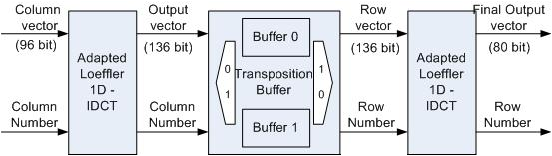
\includegraphics[width=14.60cm]{figuras/three_modules_idct.png}
\caption{The three modules 1D-IDCT, Buffer, 1D-IDCT \label{fig:idct_module}}
\end{center}
\end{figure*}

In the first Loeffer's 1D-IDCT block, the data format is a 96 bits vector, divided as eight inputs of signed 12 bits integers, and the output is formed by 17 bits integers, to explore the multipliers maximum performance.

As can be observed in Figure \ref{fig:idct_module}, the output of the first module feeds a transposition buffer. This intermediary buffer's goal is to rearrange the first module output data, oriented in columns, in a transposed matrix, oriented in rows, and supply correct input data to the second Loeffler transform.

As the buffer stores transposed information, the first line is available just after the processing of an entire matrix. Then, to keep two IDCT modules operating in parallel, writing and reading, a second buffer is used.

While the second IDCT module reads data from buffer ``0'', the first IDCT module write its processed data on buffer ``1''. For the next matrix, occurs an inversion of this process (second IDCT reading from buffer ``1'' and first IDCT writing in buffer ``0''), and the system works in a continuous and synchronous process.

The second 1D-IDCT operates as the first one, and has the same internal organization. The differences between both 1D-IDCTs modules are related with precision and data format (considering input and output). In our implementation, adjustments have been made in order to fit the results in accordance with IEEE Reference Implementation (REFERENCIA IEEE, 1991).

The input of the second IDCT has the same data format of the first IDCT's output, and the same occurs with the transposition buffer (input/output), which is a 136 bits vector, divided as eight 17 bits signed integers.

The final output is an 80 bits vector, composed by eight 10 bits signed integers.

The original Loeffler's implementation performed the calculations in four steps. To reach a better performance, and to exploit the advantages of a dedicated application, our implementation adapted each step to perform a pipelined architecture, as illustrated in Figure \label{fig:idct_4_stages_module}. Therefore, each calculation step is performed in a 4-stage pipeline. That means that while one column is ready in the output, other three columns have already been partially processed in parallel inside different pipeline stages.

\begin{figure}[!hbt]
\begin{center}

\includegraphics[height=2.16cm]{figuras/no_figure.png}
\caption{4-stage pipeline in IDCT algorithm. \label{fig:idct_4_stages_module}}
\end{center}
\end{figure}

In a global analysis of the 2D-IDCT module operation, if we assume eight columns for one data block and empty pipeline, the first row is ready at the output after seventeen pulses, and the next seven rows came in sequence (one row by each clock). It represents a total latency of 24 cycles to process an entire matrix. With full pipeline operation, the system output deliver one row for cycle and a full matrix is available every eight pulses of clock, greatly improving the overall system's performance.

%-------------------------------------------------------------------------------
\section{Result Analisys}
\label{results}

In order to compare the advantages of the proposed approach with a traditional one, this section presents the results obtained after the Computational Module implementation using both methods: the traditional one and the proposed one.

%-------------------------------------------------------------------------------
\subsection{Decompression Module}

To compare the equivalent to the Decompression Module design in FPGA, we used the implementation described by \cite{FROHLICH:2005} summarized in the Table \ref{tab:implementation_results_classic}.

\begin{table}[!hbt]
\begin{center}
\begin{tabular}{|c|c|c|c|}
\hline 
  &  1 &  Registers & Frequency (MHz) \\
\hline 
 VLD - Huff. & & ? & 200,5\\ 
\hline 
 VLD - RLE & & ? & 73,5 \\ 
\hline 
 iScan & & ? & 73,4 \\ 
\hline 
 iQuant & & ? & 85,5 \\ 
\hline 
 TOTAL & & ? & 73,5 \\ 
\hline 
\end{tabular}
\end{center}
\caption{Computational Module Implementation results in the traditional method \label{tab:implementation_results_classic}}
\end{table}

The same parameters obtained for our proposed approach are presented in Table \ref{tab:implementation_results_proposed}. As expected due to extensive use of parallelism to improve performance, the occupation area is much higher than in the traditional sequential approach, however, in terms of operation rate, our method presented a performance almost 80\% superior, which is essential to support HD video decoding.

\begin{table}[!hbt]
\begin{center}
\begin{tabular}{|c|c|c|c|}
\hline 
  & Logic Cells &  Registers & Frequency \\ 
  &  & & (MHz) \\
\hline 
 Decompression & 8556 & ? & 130,5\\ 
\hline 
\end{tabular}
\end{center}
\caption{Computational Module Implementation results in the proposed approach \label{tab:implementation_results_proposed}}
\end{table}

%-------------------------------------------------------------------------------
\subsection{IDCT Module}

The proposed method was developed in VHDL language and implemented in a Xilinx Virtex II Pro XC2VP30 FPGA. After synthesis, a total number of 24 internal multiplier blocks were used, and the obtained outputs met IEEE 1180 IDCT test specifications \cite{IEEESTD1180}, in all tests.

\begin{figure}[!hbt]
\begin{center}
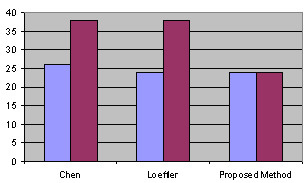
\includegraphics[height=4.84cm, width=8.04cm]{figuras/graphic_comparison_chen_loefler_proposed.png}
\caption{Graphic comparison of IDCT methods. \label{idct_graphic_compare}}
\end{center}
\end{figure}

This block was also compared with the traditional approach, and the results are shown in Table \ref{tab:idct_results_proposed}. Again the occupied chip area was bigger than the traditional IDCT, however, the performance is better due to the new proposed architecture.

\begin{table}[!hbt]
\begin{center}
\begin{tabular}{|c|c|c|c|}
\hline 
  & Logic Cells &  Registers & Frequency \\ 
  &  & & (MHz) \\
\hline 
Traditional & 8023 & 1837 & ?\\ 
IDCT & & & \\
\hline 
Proposed & 20460 & 5046 & ? \\
IDCT & & & \\
\hline 
\end{tabular}
\end{center}
\caption{IDCT results in both approaches. \label{tab:idct_results_proposed}}
\end{table}

We also compared the pipelined block described in this paper and two other IDCT hardware implementations: Chen method~\cite{CHEN:1977} and a direct implementation of Loeffler IDCT~\cite{LOEFFLER:1989}. The results are presented in Figure 7, showing that our method requires about the same number of multipliers, but performs much better, having a smaller latency compared to both other methods.

%-------------------------------------------------------------------------------
%\subsection{Lessons Learned}

%%% How the better one was implemented
%%% How the system blocks were identified
%A human analysis showed that a better implementation could be achieved...

%%% What is different in this architecture
%%% compares this architecture with to the other

%%% performance comparison
%%% this was implmented in HW too? if yes, fpga area comparison
%%% easily reusable?
%%% this process can be done in others components?
%-------------------------------------------------------------------------------
\section{Conclusion}

%%% what made possible a better implementation than AOSD
%%% Why the traditional domain decomposition methodologies didn't help the developer to idenficate a intrinsic parallelism...

This work presented a new approach to hardware implementation of the Computational  Module for use in Standard and High Definition MPEG decoders.
The authors implemented the Computational Module in the traditional approach and in the new approach, comparing both of them in terms of occupied chip area and reachable maximum performance.
Both implementations met the IEEE quality criteria for the application, while at the same time reduced 10\% of the chip area and increased almost 80\% in the overall throughput.

%%% methodologies leads to an agregation of components based on previous domain knowledge
The traditional approach used AOSD methodology to desing the MPEG decoder. This methodology failed in finding the best solution for the problem, as showed. Not only AOSD methodology but most methodologies nowadays, carry through a system domain decomposition based on previous domain knowledge, leading the system to a "agregation" of components.

%%% different components could be assembled and result in a better performance
We showed that different components, identified during classical domain decomposition phase, could be assembled in one and result in better performance. Parallel characteristics present in hardware systems aren't completely used when buiding a system with spread components.

%%% is really worth use component domain decomposition?
The performance obtained assembling different components is significant in embedded systems world. Based on the better performance achieved, we wonder if components domain decomposition, extremely employed in many methodologies, is really the best way to embedded systems design.

%-------------------------------------------------------------------------------
\section{Acknowledgements}

We would like to thanks the Digital Television Brazilian System for the financial support and the LISHA team for good times and for support...

%-------------------------------------------------------------------------------
\nocite{*}
\bibliographystyle{plain}
\bibliography{all_references}
\end{document}
